Fissata la lente sulla guida abbiamo fatto variare la posizione della candela $11$ volte, registrando in corrispondenza di ognuna il range $Q'$ di valori entro cui l'immagine dello schermo appare nitida. Indichiamo con $p$ e $q$ rispettivamente:

\begin{itemize}
	\item \textbf{p}: La posizione della fonte luminosa dalla lente;
	\item \textbf{q}: La posizione dello schermo dalla lente.
\end{itemize}

La lente è stata posizionata sulla guida ottica sul punto:
\begin{equation}
	P_{lente} = (119.00\pm 0.05)\ cm
\end{equation}
Il valore è stato ottenuto mediante una misurazione diretta e l'incertezza associata è pertanto quella strumentale. Per il calcolo di $p$ procediamo nel seguente modo:

\begin{enumerate}
	\item Posizioniamo la candela sulla guida ottica;
	\item Il valore è stato ottenuto mediante una misurazione diretta e l'incertezza associata è pertanto 	quella strumentale;
	\item Valutiamo la distanza tra questo punto e $P_{lente}$ ottenendo il valore di $p$:
	\begin{equation}
		p=P_{candela} - P_{lente}
	\end{equation}
	e la sua incertezza:
	\begin{equation}
		\Delta p = \Delta P_{candela} + \Delta P_{lente}
	\end{equation}
	Per l'incertezza vedi Legge (17).
\end{enumerate}

Per il calcolo di $q$ procediamo nel seguente modo:

\begin{enumerate}
	\item Posizioniamo lo schermo sulla guida ottica;
	\item Misuriamo il range $Q'=[Q'_{min},\ Q'_{max}]$;
	\item I valori sono stati ottenuti mediante misurazioni dirette e l'incertezza associata è pertanto quella strumentale;
	\item Calcoliamo una stima $q'$ della posizione dello schermo alla quale si osserva un'immagine nitida nel seguente modo:
	\begin{equation}
		q'=\frac{Q'_{max}+Q'_{min}}{2}
	\end{equation}
	e la sua incertezza è data dalla semidispersione:
	\begin{equation}
		\Delta q'= \frac{Q'_{max}-Q'_{min}}{2}
	\end{equation}
	\item La distanza $q$ tra lo schermo e la lente è infine ottenuta nel seguente modo:
	\begin{equation}
		q = P_{lente} - q'
	\end{equation}
	e la sua incertezza è:
	\begin{equation}
		\Delta q = \Delta P_{lente} + \Delta q'
	\end{equation}
	Per l'incertezza vedi Legge (17).
\end{enumerate}



\subsection{MISURAZIONE 1}
\begin{itemize}
	\item $P_{candela}=(149.00\pm 0.05)\ cm$
	\item $p = (30.00\pm 0.10)\ cm$
	\item $Q' = [80.00,\ 81.50]\ cm$
	\item $q = (38.2\pm 0.8)\ cm$
\end{itemize}

\subsection{MISURAZIONE 2}
\begin{itemize}
	\item $P_{candela}=(151.00\pm 0.05)\ cm$
	\item $p = (32.00\pm 0.10)\ cm$
	\item $Q' = [83.30,\ 83.70]\ cm$
	\item $q = (35.5\pm 0.2)\ cm$
\end{itemize}

\subsection{MISURAZIONE 3}
\begin{itemize}
	\item $P_{candela}=(153.00\pm 0.05)\ cm$
	\item $p = (34.00\pm 0.10)\ cm$
	\item $Q' = [85.40,\ 85.80]\ cm$
	\item $q = (33.4\pm 0.2)\ cm$
\end{itemize}

\subsection{MISURAZIONE 4}
\begin{itemize}
	\item $P_{candela}=(155.00\pm 0.05)\ cm$
	\item $p = (36.00\pm 0.10)\ cm$
	\item $Q' = [86.50,\ 87.00]\ cm$
	\item $q = (32.2\pm 0.2)\ cm$
\end{itemize}

\subsection{MISURAZIONE 5}
\begin{itemize}
	\item $P_{candela}=(157.00\pm 0.05)\ cm$
	\item $p = (38.00\pm 0.10)\ cm$
	\item $Q' = [88.10,\ 88.50]\ cm$
	\item $q = (30.7\pm 0.2)\ cm$
\end{itemize}

\subsection{MISURAZIONE 6}
\begin{itemize}
	\item $P_{candela}=(159.00\pm 0.05)\ cm$
	\item $p = (40.00\pm 0.10)\ cm$
	\item $Q' = [88.90,\ 89.50]\ cm$
	\item $q = (29.8\pm 0.3)\ cm$
\end{itemize}

\subsection{MISURAZIONE 7}
\begin{itemize}
	\item $P_{candela}=(161.00\pm 0.05)\ cm$
	\item $p = (42.00\pm 0.10)\ cm$
	\item $Q' = [89.70,\ 90.10]\ cm$
	\item $q = (29.1\pm 0.2)\ cm$
\end{itemize}

\subsection{MISURAZIONE 8}
\begin{itemize}
	\item $P_{candela}=(163.00\pm 0.05)\ cm$
	\item $p = (44.00\pm 0.10)\ cm$
	\item $Q' = [90.40,\ 91.00]\ cm$
	\item $q = (28.3\pm 0.3)\ cm$
\end{itemize}

\subsection{MISURAZIONE 9}
\begin{itemize}
	\item $P_{candela}=(165.00\pm 0.05)\ cm$
	\item $p = (46.00\pm 0.10)\ cm$
	\item $Q' = [91.30,\ 91.70]\ cm$
	\item $q = (27.5\pm 0.2)\ cm$
\end{itemize}

\subsection{MISURAZIONE 10}
\begin{itemize}
	\item $P_{candela}=(167.00\pm 0.05)\ cm$
	\item $p = (48.00\pm 0.10)\ cm$
	\item $Q' = [91.70,\ 92.30]\ cm$
	\item $q = (27.0\pm 0.3)\ cm$
\end{itemize}

\subsection{MISURAZIONE 11}
\begin{itemize}
	\item $P_{candela}=(169.00\pm 0.05)\ cm$
	\item $p = (50.00\pm 0.10)\ cm$
	\item $Q' = [92.30,\ 92.80]\ cm$
	\item $q = (26.4\pm 0.2)\ cm$
\end{itemize}

La Legge (1) descrive una relazione lineare tra i valori $\frac{1}{p}$ e $\frac{1}{q}$, che possiamo stimare mediante una regressione lineare. Dalla retta di best-fit ricaviamo infine una stima per $\frac{1}{f}$ con relativa incertezza, secondo quanto descritto nella Sezione (2.1). Ricordiamo che l'incertezza relativa a $\frac{1}{p}$ e $\frac{1}{q}$ è data dalla Legge (11), che diventa per le espressioni del tipo $\frac{1}{x}$:
\begin{equation}
	\Delta x= \frac{1}{x^2}\Delta x
\end{equation}

\begin{figure}[H]
	\centering
	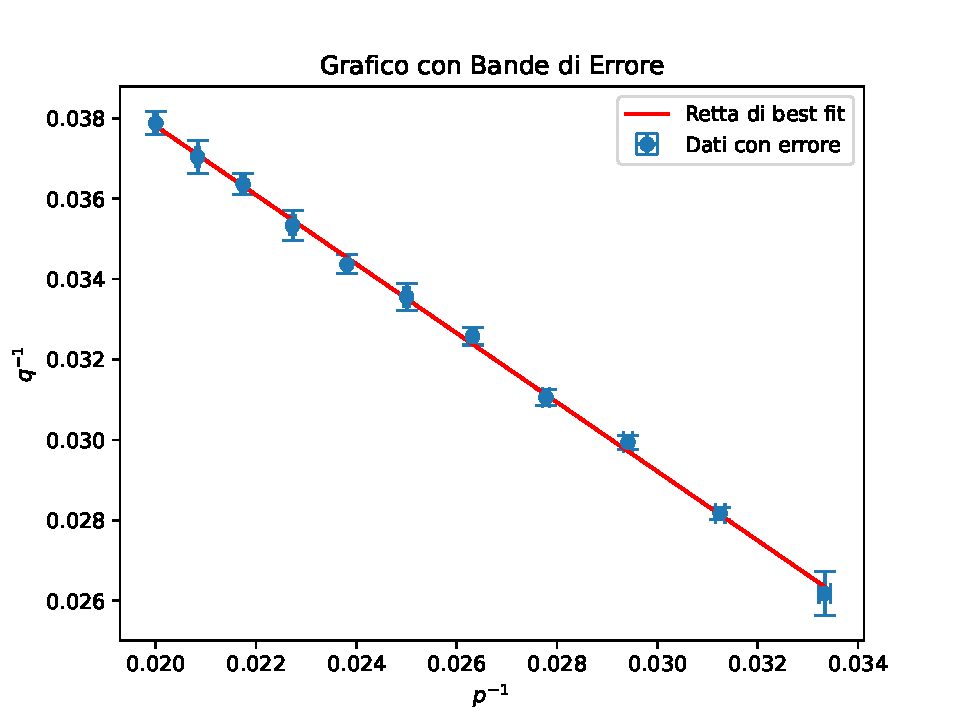
\includegraphics[width=1\textwidth]{./grafico1.pdf}
	\caption{$b=(-0.860\pm 0.031)$, 
			 $a=(0.055\pm 0.001)\ cm^{-1}$}
\end{figure}
